The survey below was written to understand the different preschool and infant-toddler programs that were present in Reggio Emilia, Parma, and Padova from the 1950's to present day. It is designed to quantify similarities and differences between the Reggio Approach and other educational programming for young children that were available to the families of each cohort. The survey focuses on administrative features and program operations; pedagogy and curricula; timing of quality improvements; variation within systems and across cities; sources of funding and costs to families; and services for immigrant families.

We administered the survey to current and retired school administrators and educative coordinators from each system in each city. Survey responses were received that allowed us to document the following programs in each decade from 1950: in Reggio Emilia, municipal and state; in Parma, municipal; and in Padova, municipal, state, and religious. Responses were also received from religious systems in Reggio Emilia and in Parma, however, they did not include historical data.

\subsection{Teacher-Child Ratios}
Although in Reggio Emilia, the teacher-child ratio for each classroom has been 2:25 since the 1960s, this number does not reflect the atelierista present at each school site, nor the pedagogista who supervises the educative staff of 4-5 schools. 

In Padova, the municipal preschool system began to consolidate in 1973, expanding from two to five sites by 1976. Teacher-child ratios for Padova's municipal preschools ranged from 1:12 to 1:24 in 1976. There were three state preschools in Padova by 1976; enrollment was relatively lower and teacher-child ratio approximately 1:15. In this same period, teacher-child ratios at religious schools ranged from 1:34-44.\footnote{This information comes from a variety of source: \citet{Reggio-Admin-data_1966-2006, Reggio-Annual-Journals_1994-2011, Padova-Admin-Data_1964-2011} and results from the survey \citep{CEHD_2016_Historical-Analysis}} 
 
\subsection{Sources of Funding and Costs to Families }
Until the early 2000s, tuition and fees to families enrolling children in religious preschools in all three cities were relatively more expensive than municipal and state programs. After the 2000s, religious schools acknowledged by the state for meeting quality components were eligible to receive state funding. Public funding across the three school systems is not equitably distributed. 

Religious schools in Padova did not receive any form of public funding in the 1970s; families were responsible for 100\% of the costs. In the 1980s and 1990s, the municipality of Padova contributed 20\% and 40\% of program costs to religious schools. In the 2000s, families paid 60\% and the remaining 40\% was shared by the state and municipality of Padova. Municipal schools in Padova are free, families pay only for meals. For state schools, families in Padova also make a voluntary contribution, usually to accommodate expenses associated with field trips.\footnote{This information is further supported by an interview with Dr. Emilia Restiglian of University of Padua.}  
 
Although eligible, the municipality of Reggio Emilia did not receive state funding for its preschool system until the 1990s and 2000s. Ironically, the municipality of Reggio Emilia contributed funds to its state schools each decade since the 1970s. Reggio Emilia also provided training for religious school teachers, beginning in 1994.  

\subsection{Overview of Survey}
Below is a list of the administrative and pedagogical components that we inquire about. Components with a * next to them are present in the Reggio Approach. Components with a $^o$ are omitted. We omit these components because we received feedback from the interviewers that those questions were interpreted differently than originally intended. These components were assembled based on published information of the Reggio Approach, and confirmed by Reggio Approach staff.\footnote{See \citet{Edwards-etal-eds_1998_Hundred-Languages} and \citet{OECD_2001_Italy-Country-Note}.}

\begin{itemize}
 \item Administrative components
 \begin{itemize}
 	\item All teachers graduated from a teacher training institution, in accordance with national guidelines.$^o$
 	\item Full-time educative coordinators, with a university degree in psychology or education, were hired by the school system.*
 	\item Educative coordinators met biweekly with educative staff to provide mentoring and professional development.*
 	\item Kitchen staff participated in professional development and routine trainings with teachers.*
 	\item Support staff participated in professional development and routine trainings with teachers.*
 	\item Teachers participated in professional development with teachers from other school systems (e.g. municipal and private Catholic).*
 	\item Schools were open daily for 8 hours.*
 	\item Schools offered extended hours for working families.*
 	\item Scheduled work hours are set aside weekly for teachers to engage families.*
 	\item Scheduled work hours are set aside weekly for teachers to document children's work.*
 	\item Scheduled work hours are set aside weekly for teachers to participate in professional development.*
 	\item Priority of enrollment is given to economically disadvantaged families.*
 	\item Priority of enrollment is given to single-parent families.*
 	\item Priority of enrollment is given to children with disabilities.*
 	\item Schools received funding from public sources.*
	\item Schools received equitable funding from public sources.$^o$
	\item Schools acquired ``paritaria'' status from the region.*$^o$
 \end{itemize}
 \item Pedagogical components
 \begin{itemize}
 	\item Daily activities were implemented by following a program to guide children in acquiring knowledge of specific concepts.
 	\item Classrooms were homogenous in age.*
 	\item Two co-teachers were assigned to the same group of children. Continuity of care provided by keeping at least one teacher with the same group from year to year.*
 	\item A full-time, on-site teacher with specific training or experience in the fine arts helped educators design creative learning activities.*
 	\item Visual arts were used as a tool to help children learn.*
 	\item Children receive religious teaching.
 	\item Teachers keep a record of children's learning.*
 	\item The design of the school environment emphasizes open spaces, natural lighting, and the use of natural materials for furniture.*
 	\item The school environment included a dedicated room where children from different classrooms work individually or in small groups.*
 	\item An on-site kitchen was used daily to prepare meals.*$^o$
 	\item Unlimited project timelines shaped the educational program.*
 	\item Academic theories of psychology and early childhood education influenced educational approaches.*
 	\item Early childhood methodologies endorsed influenced the daily program.*
 	\item Educational practices promoted by Loris Malaguzzi for early childhood influenced the daily program.*
 	\item The educational program is designed to promote good morals of family life, and is based on love of family and the homeland.
 	\item Parental boards or advisory groups were encouraged and active participants in school culture.*
	\item Transitions between schools were supported by teacher visits to homes or scheduled visits for children to new schools.$^o$
 \end{itemize}
 \end{itemize}

\subsection{Full Survey}

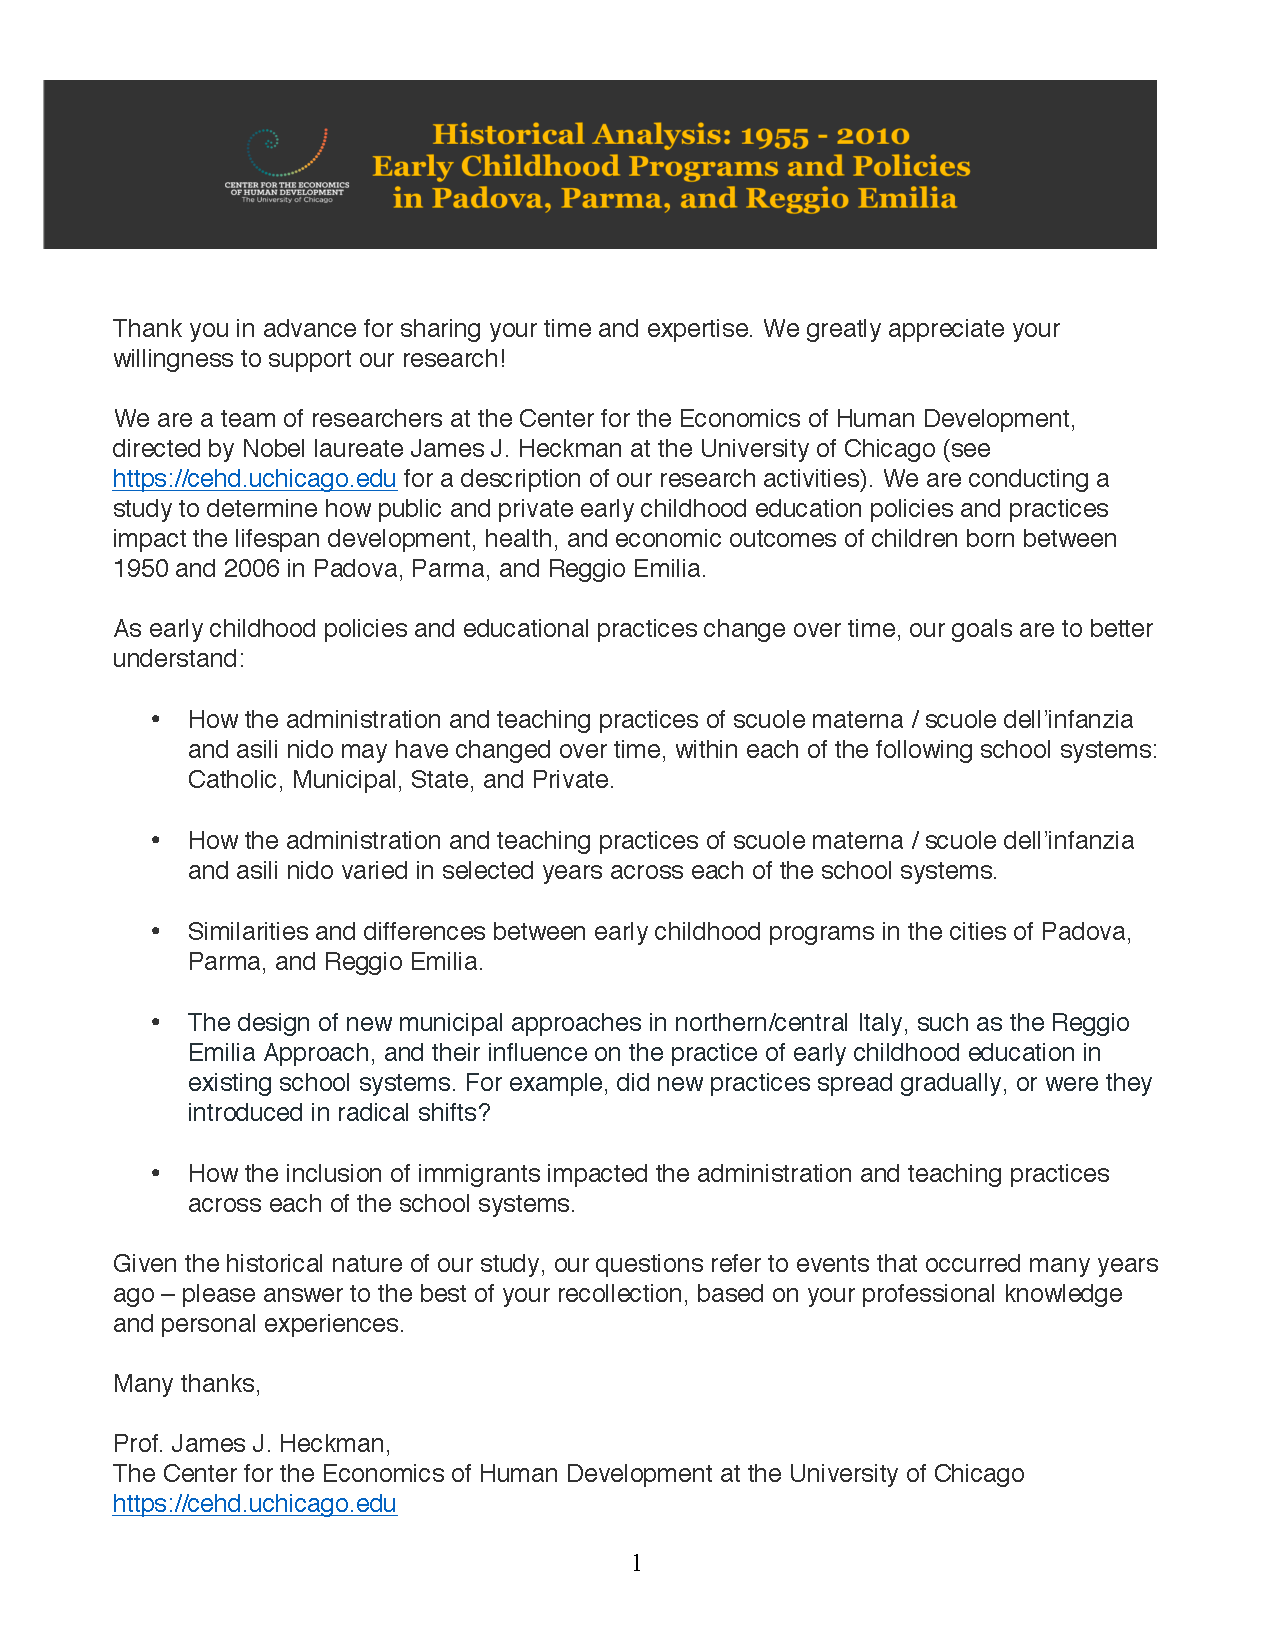
\includepdf[pages=-]{section/CEHD-ECE-Italy_SurveyQuestionnaire-ENGLISH_2016-10-24_sk}